\documentclass[11pt]{article}
\setlength{\parindent}{0pt}
\setlength{\parskip}{0.2em} % Adjust '1em' to your preference

\usepackage{geometry}
\geometry{margin=1in}

\usepackage{times}  % DO NOT CHANGE THIS
\usepackage{helvet}  % DO NOT CHANGE THIS

\usepackage{graphicx}

\usepackage[utf8]{inputenc}
\usepackage[english]{babel}
\usepackage{hyperref}
\usepackage{natbib}
\bibliographystyle{plainnat}

\usepackage{xcolor}
\newcommand{\todo}[1]{{\color{orange}{TODO: #1}}}
\newcommand{\note}[1]{{\color{blue}{NOTE: #1}}}
\newcommand{\gur}[1]{{\color{teal}{Gur: #1}}}
\newcommand{\yarden}[1]{{\color{magenta}{Yarden: #1}}}


\title{The Effect of Age of Enrollment on the Probability of Graduating in Courses}
\author{Gur Keinan 213635899 \and Yarden Adi 212585848}
\date{October 30, 2024}


\begin{document}

\maketitle

\begin{abstract}
    Many adolescents worldwide have wondered when they should start their journey in higher education. The writers of this project themselves had decided long ago to join the 'Atuda' program, which means starting university at the relatively young age of eighteen. Thus, it is natural to wonder - does the student's age at the start of learning at the university affect the success of the student? An answer to this question can drastically change the landscape of the campuses worldwide and the grades of those studying there. In this causal inference project, we aim to explore precisely that. Specifically, we investigate the following causal question: \emph{What is the causal effect of being an adult student (over 21) on the probability of completing academic courses?} Throughout this project, we present and explore the data we use to tackle this question and determine its suitability for causal analysis tasks, formally present the methods we use to answer the research question, present and discuss the analysis results, and conclude the project. One can find all of the resources used in the project in this \href{https://github.com/GurKeinan/Causal-Inference-Project-Effect-of-Age-on-Graduating}{GitHub repository}.
\end{abstract}

\textbf{Note on AI Usage:} We did not use generative AI to write this report. We only used ChatGPT, Claude, and Grammarly for revisions and corrections of our own writing.

\section{Data Review and Preprocessing}

\gur{Opening sentence.}

\subsection{Data Review}

The data used in our project originated from research done in Portugal by the \href{https://www.ipportalegre.pt/pt/}{Polytechnic Institute of Portalegre} (\gur{Equivalent to college}), as an attempt to provide information to the tutoring team about the risk of students' dropout and failure \citep{data7110146}. Commonly, it is used to build machine learning models for predicting academic performance and dropout (see relevant \href{https://www.kaggle.com/datasets/ankanhore545/dropout-or-academic-success/data}{Kaggle competitions in this subject}).

The data contains information about students' pre-academic background, age, academic performance, social and economic status, and other relevant variables. It consists of 4424 records and 37 variables \todo{number of categorical and numerical}, including the enrollment age. The dataset includes a trinary outcome variable indicating whether a student dropped out, graduated, or is still enrolled in the course. 

The data was created by joining 3 primary data sources: 
\begin{enumerate}
    \item CNAES (National Competition for Access to Higher Education) - contains information about students' academic backgrounds, demographics, and course applications at the time of their enrollment in Portuguese higher education institutions.
    \item AMS (Academic Management System) - provides student records data, including demographic information, course enrollments, and academic performance throughout their studies.
    \item PORDATA (Contemporary Portugal Database) - provides macroeconomic data, including unemployment, inflation, and GDP figures.
\end{enumerate}

\gur{Division of the data to classes like in table in the paper}


\todo{Figure star of treatment and target distributions, discussion.}

\todo{Age limitation in Portugal. We can mention and cite the fact that Portugal is said to welcome education in all ages. This statement is commonly used regarding older people, but still.}

\subsection{Data Preprocessing}

\paragraph{Treatment and Target variables} Following our causal question, we introduce a new binary variable - "being over 21". This variable acts as the \emph{treatment variable} in our analysis. We omit the numerical age variable for the rest of the analysis. Additionally, as our question focuses on the probability of completing academic courses, we introduce another binary variable - "Graduated from the course" rather than the commonly used trinary variable - "graduate/  enrolled/ dropout". This variable is the \emph{target variable} in our analysis.

\paragraph{Post-treatment variables} The dataset contains multiple records of students' academic accomplishments during their first year of higher education. Although informative for machine learning models trying to predict academic dropout, these accomplishments were recorded after the treatment was determined and, therefore, cannot be safely used in the causal inference procedure. We removed such variables, 

\paragraph{Clustering categorical values} The dataset is of impressive complexity and detail, as evident by the categorical variables with over 30 unique values. To perform meaningful analysis, we manually cluster similar categories into one broader category to represent them instead of simply removing the less frequent value. For example, we merged the values 'Armed Forces Professions', 'Armed Forces Officers', and 'Armed Forces Sergeants' into a single 'Armed Forces' value. We performed this procedure on five variables within the data set - the qualifications and occupations of the parents (mother and father) and the student's previous qualifications. 

\paragraph{Pruning categorical outliers} Even after performing the previous step, some variables still contained rare values. After careful consideration and visual inspections, we decided to prune some of the rare values to ease the analysis. Among the rest, the pruning resulted in only subjects with Portuguese nationality, \gur{detail here more}.

\paragraph{Scaling numerical variables} \todo{Add this step.}

\paragraph{One-hot encoding} \todo{Add this step.}

\section{Assumptions for Causal Inference}

In this section, we formally present and discuss four assumptions regarding the nature of our data. Combined, those assumptions guarantee the trustworthiness of an observational causal experiment's results.

\subsection{Stable Unit Treatment Value Assumption (SUTVA)}

The SUTVA assumption states that the potential outcomes of each unit are not affected by the treatment assignment of any other unit. This assumption is violated when there is interference between units, i.e., when the treatment of one unit affects the potential outcomes of other units. For example, if a treatment is a vaccine that prevents the spread of a disease, then the treatment of one individual can affect the potential outcomes of other individuals, as one individual's treatment can prevent the disease from spreading to others. In this case, the SUTVA assumption is violated.

\todo{In our data...}

\subsection{Consistency}

The consistency assumption states that an individual's potential outcome under his or her observed exposure history is the outcome that will actually be observed for that person. Put formally, for a unit that receives treatment $T$, we observe the corresponding potential outcome $Y = TY_1 + (1-T)Y_0$. This assumption can be violated when the individual's history is misreported \gur{(e.g., "Have you ever tried LSD?)}.

Our data originated from credible and regulated sources using careful and documented manipulations. Thus, we argue that the consistency assumption holds in our data.

\subsection{Ignorability - no unmeasured confounders}

The ignorability assumption states that the treatment assignment $T$ is independent of the potential outcomes $Y_0, Y_1$ given the observed covariates $X$, i.e., $Y_0, Y_1 \perp T \ | \ X$. 

\gur{'Unverifiable assumption.' https://www.ncbi.nlm.nih.gov/pmc/articles/PMC10666970/}

\gur{'We close with a reminder to readers of the optimistic view of the complexity of data and how correlation between observed variables and unmeasured ones can reduce any bias associated with unmeasured information.' https://www.ncbi.nlm.nih.gov/pmc/articles/PMC10666970/}

This assumption can always be violated since it is impossible to effectively record or scrape all relevant data for the experiment. 

\subsection{Common support (overlap)}

The common support assumption states that each unit has a non-zero probability of receiving each treatment level, i.e., $\forall x \in X, P(T=1|X=x) > 0$ and $P(T=0|X=x) > 0$.

We empirically validate this assumption using propensity scores. We trained a logistic regression model to predict the treatment assignment based on the covariates, and used the predicted probabilities as the propensity scores. We then plotted the propensity scores of the treated and control groups to ensure that there is a significant overlap between the two groups. The results are presented in Figure \ref{fig:common_support}. The lowest predicted propensity score of the treated group is $0.0053$, and of the control group is $0.0018$. Therefore, we conclude that the common support assumption holds in our data.

\begin{figure}
    \centering
    \caption{Common support of the propensity scores}
    \label{fig:common_support}
    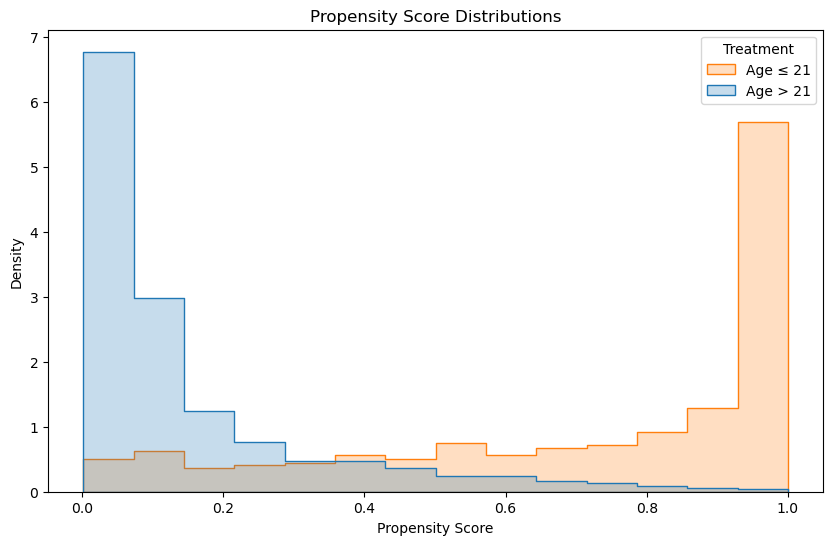
\includegraphics[width = 0.8\textwidth]{images/common support propensity graph.png}
\end{figure}



\section{Causal Analysis Methodology}

After validating the assumptions for causal inference, we proceed to describe the methodology we use to perform the causal analysis. This methodology is based on the potential outcomes framework and the assumptions we discussed in the previous section. We now present the relevant measures and the methods we use to estimate them and their confidence intervals.

\subsection{Measures}

In order to quantify the causal effect of the treatment on the outcome, one usually tries to estimate the Average Treatment Effect (ATE). However, in some cases, it is more informative to estimate the Average Treatment Effect on the Treated (ATT) or the Average Treatment Effect on the Control (ATC). We now formally define these measures.

\paragraph{Average Treatment Effect (ATE)} The Average Treatment Effect is the difference between the expected outcome under treatment and the expected outcome under control. Formally, it is defined as $ATE = E[Y_1 - Y_0]$.

\paragraph{Average Treatment Effect on the Treated (ATT)} The Average Treatment Effect on the Treated is the difference between the expected outcome under treatment and the expected outcome under control, but only for the treated units. Formally, it is defined as $ATT = E[Y_1 - Y_0 | T = 1]$. 

\paragraph{Average Treatment Effect on the Control (ATC)} The Average Treatment Effect on the Control is the difference between the expected outcome under treatment and the expected outcome under control, but only for the control units. Formally, it is defined as $ATC = E[Y_1 - Y_0 | T = 0]$. 

Each of the three measures provides a different perspective on the causal effect of the treatment. The ATE measures the average effect of the treatment on the entire population, while the ATT and ATC measures provide insights into the effect of the treatment on the treated and control units, respectively. The ATT and ATC measures are particularly useful when the treatment assignment is not controlled (not random), as is the case in observational studies.

\subsection{Methods}

\gur{Maybe covariates adjustment, IPW, Doubly Robust, Matching, one more sophisticated method. (the first 3 have nice rhythm together).}

We now present the methods we use to estimate the causal effect of the treatment on the outcome. We also detail about the implementation of these methods and the relevant hyperparameters.

\subsubsection{Doubly Robust Estimation}

Doubly Robust Estimation is a method that combines the outcome regression and propensity score weighting methods to estimate the causal effect of the treatment. Formally, given the observed outcome $Y$, the treatment assignment $T$, and the covariates $X$, the Doubly Robust Estimator is defined as:

\gur{Add the formula here.}

Where $\hat{\mu}_1$ and $\hat{\mu}_0$ are the outcome regression models for the treated and control units, respectively, and $\hat{e}(X_i)$ is the estimated propensity score model. The Doubly Robust Estimator is not biased if either the outcome regression model or the propensity score model is correctly specified, making it a robust method for estimating causal effect.

\paragraph{Implementation Details} \todo{Details about the implementation of the Doubly Robust Estimator.}


\subsubsection{Propensity Score Matching}

Propensity Score Matching is a method that matches treated and control units based on their propensity scores, which are the estimated probabilities of receiving the treatment given the covariates. The matching process aims to create groups of treated and control units that are similar in terms of their propensity scores, thus creating a balanced dataset. After matching the units, the causal effect of the treatment can be estimated by averaging the differences in outcomes between the matched treated and control units.

\paragraph{Implementation Details} \todo{Details about the implementation of Propensity Score Matching.}





\subsection{Bootstrap Confidence Intervals}








\section{Results}

\begin{itemize}
    \item One graph to compare all of the results from the methods (box plots).
    \item Discussion.
    \item Analyze correlation / dominant features.
\end{itemize}

\section{Discussion}

\begin{itemize}
    \item Conclusions
    \item Possible weaknesses.
    \item Avenues for future work.
\end{itemize}

\bibliography{references.bib}

\appendix

\end{document}